\chapter{Metodologia}
\label{chap:metodologia}


\section{Fundamentação teórica}
\label{sec:fundamentacao}

\begin{equation}
\mathbf{B}(x, y, z) = - \nabla \Gamma(x, y, z)
\label{eq:B-true-generic}
\end{equation}

\begin{equation}
\Gamma(x, y, z) = - \gamma_{m} \iiint\limits_{\upsilon} \mathbf{m}(x', y', z') \cdot \nabla\frac{1}{r'} 
\; d\upsilon'
\label{eq:Gamma-potential}
\end{equation}

\begin{equation}
\frac{1}{r'} = \frac{1}{\left[ (x - x')^{2} + (y - y')^{2} + (z - z')^{2} \right]^{\frac{1}{2}}}
\label{eq:inv-r'}
\end{equation}

\begin{equation}
\mathbf{m}(x', y', z') = \begin{bmatrix}
m_{x}(x', y', z') \\
m_{y}(x', y', z') \\
m_{z}(x', y', z')
\end{bmatrix}
\label{eq:mag-vector-true-generic}
\end{equation}

\begin{equation}
B_{\alpha}(x, y, z) = \gamma_{m} \iiint\limits_{\upsilon} 
\mathbf{m}(x', y', z') \cdot \partial_{\alpha} \nabla \frac{1}{r'} 
\; d\upsilon' \: , \quad \alpha = x, y, z \: ,
\label{eq:B-alpha-true-generic}
\end{equation}
em que $\partial_{\alpha} \equiv \frac{\partial}{\partial \alpha}$ ...

Presumindo que, em qualquer ponto $(x, y, z)$ fora das fontes magnéticas, nenhuma 
componente $B_{\alpha}(x, y, z)$ (equação \ref{eq:B-alpha-true-generic}) varia no tempo, 
o campo de indução magnética $\mathbf{B}(x, y, z)$ (equação \ref{eq:B-true-generic}) é governado
pela lei de Gauss
\begin{equation}
\nabla \cdot \mathbf{B}(x, y, z) = 
\partial_{x} B_{x}(x, y, z) + \partial_{y} B_{y}(x, y, z) + \partial_{z} B_{z}(x, y, z) = 
0
\label{eq:lei-Gauss}
\end{equation}
e a lei de Ampère
\begin{equation}
\nabla \times \mathbf{B}(x, y, z) = \begin{bmatrix}
\partial_{y} B_{z}(x, y, z) - \partial_{z} B_{y}(x, y, z) \\
\partial_{z} B_{x}(x, y, z) - \partial_{x} B_{z}(x, y, z) \\
\partial_{x} B_{y}(x, y, z) - \partial_{y} B_{x}(x, y, z) 
\end{bmatrix} = 
\begin{bmatrix}
0 \\
0 \\
0
\end{bmatrix} \: .
\label{eq:lei-Ampere}
\end{equation}



Considere o vetor unitário 
\begin{equation}
\hat{\mathbf{u}}(I, D) = 
\begin{bmatrix}
\hat{u}_{x}(I, D) \\
\hat{u}_{y}(I, D) \\
\hat{u}_{z}(I, D) 
\end{bmatrix} = 
\begin{bmatrix}
\cos I \, \cos D \\
\cos I \, \sin D \\
\sin I
\end{bmatrix} \: ,
\label{eq:u-hat}
\end{equation}
definido em termos de uma inclinação $I$ e uma declinação $D$.


\begin{equation}
\Delta T(x, y, z) = \hat{\mathbf{u}}(I_{0}, D_{0}) \cdot \mathbf{B}(x, y, z) \: .
\label{eq:Delta-T-true}
\end{equation}


\section{Camada equivalente magnética}
\label{sec:camada-equivalente}


\begin{equation}
\tilde{\mathbf{B}}(x, y, z) = - \nabla \Phi(x, y, z)
\label{eq:B-layer}
\end{equation}

\begin{equation}
\Phi(x, y, z) = - \gamma_{m} \int\limits_{-\infty}^{+\infty}\int\limits_{-\infty}^{+\infty} 
p(x'', y'', z_{c}) \, \hat{\mathbf{u}}(I, D) \cdot \nabla \frac{1}{r''} \; dS'' \: , \quad z_{c} > z \: ,
\label{eq:Phi-potential}
\end{equation}

\begin{equation}
\frac{1}{r''} = \frac{1}{\left[ (x - x'')^{2} + (y - y'')^{2} + (z - z_{c})^{2} \right]^{\frac{1}{2}}}
\label{eq:inv-r''}
\end{equation}

\begin{equation}
\tilde{B}_{\alpha}(x, y, z) = \gamma_{m} \int\limits_{-\infty}^{+\infty}\int\limits_{-\infty}^{+\infty} 
p(x'', y'', z_{c}) \, \hat{\mathbf{u}}(I, D) \cdot \partial_{\alpha} \nabla \frac{1}{r''} \; dS'' 
\: , \quad \alpha = x, y, z \: ,
\label{eq:B-alpha-layer}
\end{equation}

\begin{equation}
\Delta\tilde{T}(x, y, z) = \hat{\mathbf{u}}(I_{0}, D_{0}) \cdot \tilde{\mathbf{B}}(x, y, z) \: .
\label{eq:Delta-T-layer}
\end{equation}


\section{Consequências das Leis de Gauss e Amp{\`e}re}
\label{sec:Gauss-Ampere}

As equações \ref{eq:B-layer}--\ref{eq:B-alpha-layer} definem o campo de indução 
magnética produzido por uma camada equivalente localizada em $z = z_{c}$,
com distribuição de intensidade de momento magnético 
$p(x'', y'', z_{c})$ e direção de magnetização uniforme definida por 
$\hat{\mathbf{u}}(I, D)$ (equação \ref{eq:u-hat}). Nesta seção, mostrarei que, 
se esta camada reproduz uma das componentes $B_{\alpha}(x, y, z)$ (equação \ref{eq:B-alpha-true-generic})
do campo de indução magnética $\mathbf{B}(x, y, z)$ (equação \ref{eq:B-true-generic}) 
produzido por um conjunto de fontes magnéticas arbitrárias em todos os pontos 
$(x, y, z)$ fora das fontes e acima da camada ($z < z_{c}$), esta mesma camada deve, 
obrigatoriamente, reproduzir as outras componentes $B_{\alpha}(x, y, z)$ do campo 
produzido pelas fontes arbitrárias.

Considere três camadas equivalentes definidas na mesma coordenada vertical $z = z_{c}$, 
com distribuições de intensidade de momento magnético 
$p(x'', y'', z_{c}) \equiv p_{(\alpha)}$ e direções de magnetização uniforme definidas por 
$\hat{\mathbf{u}}^{(\alpha)} \equiv \hat{\mathbf{u}}(I_{(\alpha)}, D_{(\alpha)})$,
com componentes Cartesianas $\hat{u}^{(\alpha)}_{\beta} \equiv \hat{u}_{\beta}(I_{(\alpha)}, D_{(\alpha)})$ 
(equação \ref{eq:u-hat}), em que $\alpha = x, y, z$, $\beta = x, y, z$. 
Considere também, momentaneamente, que cada camada $\alpha$ produz a componente 
$\breve{B}_{\alpha}(x, y, z)$ de um mesmo campo de indução magnética $\breve{\mathbf{B}}(x, y, z)$, 
tal que:
\begin{equation}
\breve{B}_{\alpha}(x, y, z) = \gamma_{m} \int\limits_{-\infty}^{+\infty}\int\limits_{-\infty}^{+\infty} 
p_{(\alpha)} \, \hat{\mathbf{u}}^{(\alpha)} \cdot \partial_{\alpha} \nabla \frac{1}{r''} \; dS'' 
\: , \quad \alpha = x, y, z \: ,
\label{eq:B-alpha-3layers}
\end{equation}
e
\begin{equation}
\breve{\mathbf{B}}(x, y, z) = \begin{bmatrix}
\breve{B}_{x}(x, y, z) \\
\breve{B}_{y}(x, y, z) \\
\breve{B}_{z}(x, y, z)
\end{bmatrix} \: .
\label{eq:B-3layers}
\end{equation}
Calculando o divergente de $\breve{\mathbf{B}}(x, y, z)$ 
e trocando a ordem das derivadas parciais, obtemos 
\begin{equation}
\nabla \cdot \breve{\mathbf{B}}(x, y, z) = I_{1} + I_{2} + I_{3} \: ,
\label{eq:divergent-layer}
\end{equation}
em que os termos são integrais de superfície dadas por
\begin{equation*}
\begin{split}
I_{1} &= \gamma_{m} \iint
p_{(x)} \hat{u}^{(x)}_{x} \partial_{xxx} \frac{1}{r''} +
p_{(y)} \hat{u}^{(y)}_{x} \partial_{yyx} \frac{1}{r''} +
p_{(z)} \hat{u}^{(z)}_{x} \partial_{zzx} \frac{1}{r''} \; dS'' \\
I_{2} &= \gamma_{m} \iint
p_{(x)} \hat{u}^{(x)}_{y} \partial_{xxy} \frac{1}{r''} +
p_{(y)} \hat{u}^{(y)}_{y} \partial_{yyy} \frac{1}{r''} +
p_{(z)} \hat{u}^{(z)}_{y} \partial_{zzy} \frac{1}{r''} \; dS'' \\
I_{3} &= \gamma_{m} \iint
p_{(x)} \hat{u}^{(x)}_{z} \partial_{xxz} \frac{1}{r''} +
p_{(y)} \hat{u}^{(y)}_{z} \partial_{yyz} \frac{1}{r''} +
p_{(z)} \hat{u}^{(z)}_{z} \partial_{zzz} \frac{1}{r''} \; dS''
\end{split} \:\: .
\end{equation*}
Por conveniência, os limites de integração $-\infty$ e $+\infty$ foram omitidos.
Sabemos que as derivadas primeiras $\partial_{\beta} \frac{1}{r''}$, $\beta = x, y, z$, de 
$\frac{1}{r''}$ (equação \ref{eq:inv-r''}) são funções harmônicas. Esta propriedade permite 
reescrever as integrais $I_{1}$, $I_{2}$ e $I_{3}$ da seguinte forma:
\begin{equation}
\begin{split}
I_{1} &= \gamma_{m} \iint
\left[ p_{(x)} \hat{u}^{(x)}_{x} - p_{(z)} \hat{u}^{(z)}_{x} \right] \partial_{xxx} \frac{1}{r''} +
\left[ p_{(y)} \hat{u}^{(y)}_{x} - p_{(z)} \hat{u}^{(z)}_{x} \right] \partial_{yyx} \frac{1}{r''} +
\; dS'' \\
I_{2} &= \gamma_{m} \iint
\left[ p_{(x)} \hat{u}^{(x)}_{y} - p_{(z)} \hat{u}^{(z)}_{y} \right] \partial_{xxy} \frac{1}{r''} +
\left[ p_{(y)} \hat{u}^{(y)}_{y} - p_{(z)} \hat{u}^{(z)}_{y} \right] \partial_{yyy} \frac{1}{r''} +
\; dS'' \\
I_{3} &= \gamma_{m} \iint
\left[ p_{(x)} \hat{u}^{(x)}_{z} - p_{(z)} \hat{u}^{(z)}_{z} \right] \partial_{xxz} \frac{1}{r''} +
\left[ p_{(y)} \hat{u}^{(y)}_{z} - p_{(z)} \hat{u}^{(z)}_{z} \right] \partial_{yyz} \frac{1}{r''} +
\; dS''
\label{eq:divergent-layer-I123}
\end{split} \:\: .
\end{equation}
Dessa forma, fica evidente que os integrandos de $I_{1}$, $I_{2}$ e $I_{3}$ (equação \ref{eq:divergent-layer-I123}) 
são combinações lineares de funções linearmente independentes, que são derivadas 
terceiras da função $\frac{1}{r''}$ (equação \ref{eq:inv-r''}).
Note que, para o campo de indução magnética $\breve{\mathbf{B}}(x, y, z)$ (equação \ref{eq:B-3layers}) 
respeitar a lei de Gauss (equação \ref{eq:lei-Gauss}), é necessário que as integrais $I_{1}$, $I_{2}$ e $I_{3}$ 
sejam todas nulas.
Para que isso aconteça sem que as distribuições de intensidade de momento magnético 
$p_{(x)}$, $p_{(y)}$ e $p_{(z)}$ sejam nulas em todos os pontos $(x'', y'', z_{c})$, é necessário 
que os termos entre colchetes
nos integrandos de $I_{1}$, $I_{2}$ e $I_{3}$ sejam nulos em todos os pontos $(x'', y'', z_{c})$.
Isso, por sua vez, só é possível se as distribuições de intensidade de momento magnético 
e as direções de magnetização uniforme das três camadas forem iguais entre si, isto é, se 
$p_{(x)} = p_{(y)} = p_{(z)}$ e 
$\hat{\mathbf{u}}^{(x)} = \hat{\mathbf{u}}^{(y)} = \hat{\mathbf{u}}^{(z)}$.
Neste caso, o campo de indução magnética produzido pela camada equivalente é descrito pelas equações 
\ref{eq:B-layer}--\ref{eq:B-alpha-layer}.

Calculando o rotacional do campo de indução magnética 
$\breve{\mathbf{B}}(x, y, z)$ (equação \ref{eq:B-3layers}) produzido pelas três camadas 
e trocando a ordem das derivadas parciais, obtemos
\begin{equation}
\nabla \times \breve{\mathbf{B}}(x, y, z) = \begin{bmatrix}
\gamma_{m} \iint
\left[ p_{(z)} \, \hat{\mathbf{u}}^{(z)} - p_{(y)} \, \hat{\mathbf{u}}^{(y)} \right] \cdot 
\partial_{yz} \nabla \frac{1}{r''} \; dS'' \\
\gamma_{m} \iint
\left[ p_{(x)} \, \hat{\mathbf{u}}^{(x)} - p_{(z)} \, \hat{\mathbf{u}}^{(z)} \right] \cdot 
\partial_{xz} \nabla \frac{1}{r''} \; dS'' \\
\gamma_{m} \iint
\left[ p_{(y)} \, \hat{\mathbf{u}}^{(y)} - p_{(x)} \, \hat{\mathbf{u}}^{(x)} \right] \cdot 
\partial_{xy} \nabla \frac{1}{r''} \; dS''
\end{bmatrix} \: .
\label{eq:curl-layer}
\end{equation}
Novamente, os limites de integração $-\infty$ e $+\infty$ foram omitidos por conveniência.
Note que os integrandos das componentes do rotacional de $\breve{\mathbf{B}}(x, y, z)$ 
(equação \ref{eq:curl-layer}) são combinações lineares de funções linearmente 
independentes, que são derivadas terceiras de $\frac{1}{r''}$ (equação \ref{eq:inv-r''}).
Sabemos que, para o campo de indução magnética $\breve{\mathbf{B}}(x, y, z)$ 
(equação \ref{eq:B-3layers}) respeitar a lei de Ampère (equação \ref{eq:lei-Ampere}), é necessário que as 
três componentes de $\nabla \times \breve{\mathbf{B}}(x, y, z)$ sejam nulas. 
Para que isso aconteça sem que as distribuições de intensidade de momento magnético 
$p_{(x)}$, $p_{(y)}$ e $p_{(z)}$ sejam 
nulas em todos os pontos $(x'', y'', z_{c})$, é necessário que os termos entre colchetes
nos integrandos da equação \ref{eq:curl-layer} sejam nulos em todos os pontos $(x'', y'', z_{c})$.
Mais uma vez, isso só é possível se as distribuições de intensidade de momento magnético 
e as direções de magnetização uniforme das três camadas forem iguais entre si, isto é, se 
$p_{(x)} = p_{(y)} = p_{(z)}$ e 
$\hat{\mathbf{u}}^{(x)} = \hat{\mathbf{u}}^{(y)} = \hat{\mathbf{u}}^{(z)}$.
Neste caso, o campo de indução magnética produzido pela camada equivalente é descrito pelas equações 
\ref{eq:B-layer}--\ref{eq:B-alpha-layer}.

De acordo com estes resultados teóricos, a hipótese de que cada componente $\breve{B}_{\alpha}(x, y, z)$ 
(equação \ref{eq:B-alpha-3layers}), $\alpha = x, y, z$, de um mesmo campo de indução magnética $\breve{\mathbf{B}}(x, y, z)$ 
(equação \ref{eq:B-3layers}) pode ser reproduzida por uma camada equivalente diferente resulta na 
violação das leis de Gauss (equação \ref{eq:lei-Gauss}) e de Ampère (equação \ref{eq:lei-Ampere}).
Isto significa que há uma única camada equivalente localizada em $z = z_{c}$, 
com uma determinada distribuição de intensidades de momento magnético $p(x'', y'', z_{c})$ e uma 
determinada direção de magnetização uniforme $\hat{\mathbf{u}}(I, D)$ capaz de reproduzir, simultaneamente,
as três componentes de um mesmo campo de indução magnética.

Considere agora a existência de uma camada equivalente localizada em $z = z_{c}$, com uma determinada 
distribuição de intensidades de momento magnético $p(x'', y'', z_{c})$ e uma determinada 
direção de magnetização uniforme $\hat{\mathbf{u}}(I, D)$, que produz um campo de indução 
magnética $\tilde{\mathbf{B}}(x, y, z)$ (equação \ref{eq:B-layer}). 
É importante ressaltar que a direção de magnetização $\hat{\mathbf{u}}(I, D)$ na camada não 
precisa ter nenhum compromisso com a direção de magnetização das fontes verdadeiras.
Adicionalmente, 
considere que uma componente $\tilde{B}_{\alpha}(x, y, z)$ (equação \ref{eq:B-alpha-layer}) 
do campo produzido por esta camada reproduz a componente $B_{\alpha}(x, y, z)$ (equação \ref{eq:B-alpha-true-generic}) 
do campo produzido por fontes magnéticas arbitrárias em todos os pontos $(x, y, z)$ localizados fora das fontes e acima 
da camada ($z < z_{c}$). Utilizando o resultado teórico exposto acima, conclui-se que 
esta mesma camada deve obrigatoriamente reproduzir as outras duas componentes do campo produzido 
pelas fontes magnéticas. Caso contrário, cada componente $\tilde{B}_{\alpha}(x, y, z)$ 
(equação \ref{eq:B-alpha-layer}) do campo produzido pela camada, e consequentemente cada componente 
$B_{\alpha}(x, y, z)$ (equação \ref{eq:B-alpha-true-generic}) do campo produzido pelas fontes arbitrárias, 
deverá ser reproduzida por uma camada equivalente diferente, o que violaria as leis de 
Gauss (equação \ref{eq:lei-Gauss}) e de Ampère (equação \ref{eq:lei-Ampere}).


\section{Distribuição de momentos positiva}
\label{sec:distribuicao-positiva}


Considere agora que o conjunto de fontes magnéticas possui direção de magnetização 
uniforme, com inclinação $I_{t}$ e declinação $D_{t}$, de tal forma que o vetor 
de magnetização total (equação \ref{eq:mag-vector-true-generic}) seja dado por:
\begin{equation}
\mathbf{m}(x', y', z') = m(x', y', z') \, \hat{\mathbf{u}}(I_{t}, D_{t}) \: ,
\label{eq:mag-vector-true-uniform}
\end{equation}
em que $m(x', y', z')$ representa a intensidade de magnetização em um ponto $(x', y', z')$ 
localizado no interior das fontes e $\hat{\mathbf{u}}(I_{t}, D_{t})$ é o vetor unitário 
definido pela equação \ref{eq:u-hat}.
Neste caso, o potencial magnético escalar $\Gamma(x, y, z)$ (equação \ref{eq:Gamma-potential}) 
e o campo de indução magnética $\mathbf{B}(x, y, z)$ (equação \ref{eq:B-true-generic}) produzidos 
pelas fontes ficam definidos por:
\begin{equation}
\Gamma(x, y, z) = - \gamma_{m} \iiint\limits_{\upsilon} 
m(x', y', z') \, \hat{\mathbf{u}}(I_{t}, D_{t}) \cdot \nabla\frac{1}{r'} 
\; d\upsilon'
\label{eq:Gamma-potential-mag-uniform}
\end{equation}
e
\begin{equation}
\mathbf{B}(x, y, z) = \gamma_{m} \, \mathbf{M}(x, y, z) \, \hat{\mathbf{u}}(I_{t}, D_{t}) \: ,
\label{eq:B-true-mag-uniform}
\end{equation}
em que $\mathbf{M}(x, y, z)$ é uma matriz dada por
\begin{equation}
	\mathbf{M}(x, y, z) = \begin{bmatrix}
		\partial_{xx} \Omega(x, y, z) & 
		\partial_{xy} \Omega(x, y, z) &
		\partial_{xz} \Omega(x, y, z) \\
		\partial_{xy} \Omega(x, y, z) & 
		\partial_{yy} \Omega(x, y, z) &
		\partial_{yz} \Omega(x, y, z) \\
		\partial_{xz} \Omega(x, y, z) & 
		\partial_{yz} \Omega(x, y, z) &
		\partial_{zz} \Omega(x, y, z)
	\end{bmatrix} \: ,
	\label{eq:M-matrix}
\end{equation}
cujos elementos $\partial_{\alpha\beta} \Omega(x, y, z) \equiv 
\frac{\partial^{2} \Omega(x, y, z)}{\partial \alpha \partial \beta}$, 
$\alpha, \beta = x, y, z$, representam as derivadas segundas da função harmônica 
\begin{equation}
\Omega(x, y, z) = \iiint\limits_{\upsilon} 
m(x', y', z') \, \frac{1}{r'} \: d\upsilon' \: ,
\label{eq:Omega-potential}
\end{equation}
sendo $\frac{1}{r'}$ definida pela equação \ref{eq:inv-r'}.
A intensidade de magnetização $m(x', y', z')$ é estritamente positiva em todos os pontos no interior das fontes. 
Por conseguinte, $\Omega(x, y, z)$ é positiva em todos os pontos exteriores a fonte magnética. Do ponto de vista físico, 
$\mathbf{M}(x, y, z)$ (equação \ref{eq:M-matrix}) e $\Omega(x, y, z)$ (equação \ref{eq:Omega-potential}) representam, 
respectivamente, o tensor gradiente e o potencial gravitacional que seriam produzidos pelas fontes magnéticas no ponto 
$(x,y,z)$, se elas tivessem distribuição de densidade proporcional a $m(x', y', z')$. Note que $\mathbf{M}(x, y, z)$ é 
uma matriz simétrica, seu traço é nulo em todos os pontos $(x,y,z)$ exteriores as fontes magnéticas e possui cinco 
componentes independentes que são funções harmônicas \citep{pedersen_rasmussen1990}. 
Usando o campo de indução magnética $\mathbf{B}(x, y, z)$ (equação \ref{eq:B-true-mag-uniform}) produzido 
por fontes magnéticas com direção de magnetização uniforme e explorando as propriedades da matriz 
$\mathbf{M}(x, y, z)$ (equação \ref{eq:M-matrix}), podemos reescrever a anomalia de campo total 
$\Delta T(x, y, z)$ (equação \ref{eq:Delta-T-true}) da seguinte forma:
\begin{equation}
	\begin{split}
		\Delta T(x, y, z) = \:
		& a_{xx} \, \partial_{xx} \Omega(x, y, z) + 
		a_{xy} \, \partial_{xy} \Omega(x, y, z) + 
		a_{xz} \, \partial_{xz} \Omega(x, y, z) + \\
		& a_{yy} \, \partial_{yy} \Omega(x, y, z) + 
		a_{yz} \, \partial_{yz} \Omega(x, y, z)
	\end{split} \quad ,
	\label{eq:Delta-T-true-mag-uniform}
\end{equation}
em que 
\begin{equation}
	\begin{split}
		a_{xx} &= \hat{u}_{x}(I_{t}, D_{t}) \hat{u}_{x}(I_{0}, D_{0}) - \hat{u}_{z}(I_{t}, D_{t}) \hat{u}_{z}(I_{0}, D_{0}) \\
		a_{xy} &= \hat{u}_{x}(I_{t}, D_{t}) \hat{u}_{y}(I_{0}, D_{0}) + \hat{u}_{y}(I_{t}, D_{t}) \hat{u}_{x}(I_{0}, D_{0}) \\
		a_{xz} &= \hat{u}_{x}(I_{t}, D_{t}) \hat{u}_{z}(I_{0}, D_{0}) + \hat{u}_{z}(I_{t}, D_{t}) \hat{u}_{x}(I_{0}, D_{0}) \\
		a_{yy} &= \hat{u}_{y}(I_{t}, D_{t}) \hat{u}_{y}(I_{0}, D_{0}) - \hat{u}_{z}(I_{t}, D_{t}) \hat{u}_{z}(I_{0}, D_{0}) \\
		a_{yz} &= \hat{u}_{y}(I_{t}, D_{t}) \hat{u}_{z}(I_{0}, D_{0}) + \hat{u}_{z}(I_{t}, D_{t}) \hat{u}_{y}(I_{0}, D_{0})
	\end{split}
\label{eq:a-coefficients-sources}
\end{equation}
são constantes definidas pelas componentes $\hat{u}_{\alpha}(I_{0}, D_{0})$ e $\hat{u}_{\beta}(I_{t}, D_{t})$, 
$\alpha = x, y, z$, $\beta = x, y, z$, dos vetores unitários $\hat{\mathbf{u}}(I_{0}, D_{0})$ e 
$\hat{\mathbf{u}}(I_{t}, D_{t})$ (equação \ref{eq:u-hat}), respectivamente,
definidos pela inclinação $I_{0}$ e declinação $D_{0}$ do campo principal na área de estudo e 
pela inclinação $I_{t}$ e declinação $D_{t}$ da magnetização uniforme das fontes magnéticas. 
Por simplicidade, omitimos a dependência dos coeficientes $a_{\alpha\beta}$ em relação aos parâmetros 
$I_{0}$, $D_{0}$, $I_{t}$ e $D_{t}$.
As equações \ref{eq:Delta-T-true-mag-uniform} e \ref{eq:a-coefficients-sources} mostram que a anomalia de campo 
total $\Delta T(x, y, z)$ produzida por fontes magnéticas com direção de magnetização uniforme é 
uma combinação linear de cinco funções harmônicas e independentes, que são derivadas segundas 
de $\Omega(x, y, z)$ (equação \ref{eq:Omega-potential}).

Considere uma camada equivalente localizada em $z = z_{c}$, com a mesma direção de magnetização 
das fontes verdadeiras e com uma distribuição de intensidades de momento magnético $p(x'', y'', z_{c})$
tal que a condição $\Delta T(x, y, z) = \Delta \tilde{T}(x, y, z)$ seja satisfeita em todos os pontos 
$(x, y, z)$ localizados fora das fontes e acima da camada ($z < z_{c}$).
Nesse caso, é possível reescrever o campo de indução magnética $\tilde{\mathbf{B}}(x, y, z)$
(equação \ref{eq:B-layer}) da seguinte forma:
\begin{equation}
\tilde{\mathbf{B}}(x, y, z) = \gamma_{m} \tilde{\mathbf{M}}(x, y, z) \hat{\mathbf{u}}(I_{t}, D_{t}) \: ,
\label{eq:B-layer-alternative}
\end{equation}
em que $\tilde{\mathbf{M}}(x, y, z)$ é uma matriz dada por
\begin{equation}
	\tilde{\mathbf{M}}(x, y, z) = \begin{bmatrix}
		\partial_{xx} \tilde{\Omega}(x, y, z) & 
		\partial_{xy} \tilde{\Omega}(x, y, z) &
		\partial_{xz} \tilde{\Omega}(x, y, z) \\
		\partial_{xy} \tilde{\Omega}(x, y, z) & 
		\partial_{yy} \tilde{\Omega}(x, y, z) &
		\partial_{yz} \tilde{\Omega}(x, y, z) \\
		\partial_{xz} \tilde{\Omega}(x, y, z) & 
		\partial_{yz} \tilde{\Omega}(x, y, z) &
		\partial_{zz} \tilde{\Omega}(x, y, z)
	\end{bmatrix} \: ,
	\label{eq:M-tilde-matrix}
\end{equation}
cujos elementos $\partial_{\alpha\beta} \tilde{\Omega}(x, y, z) \equiv 
\frac{\partial^{2} \tilde{\Omega}(x, y, z)}{\partial \alpha \partial \beta}$, 
$\alpha, \beta = x, y, z$, representam as derivadas segundas da função harmônica 
\begin{equation}
\tilde{\Omega}(x, y, z) = \int\limits_{-\infty}^{+\infty}\int\limits_{-\infty}^{+\infty} 
p(x'', y'', z_{c}) \, \frac{1}{r''} \: dS'' \: , \quad z < z_{c} \: ,
\label{eq:Omega-tilde-potential}
\end{equation}
sendo $\frac{1}{r''}$ definida pela equação \ref{eq:inv-r''}.
Note que $\tilde{\mathbf{M}}(x, y, z)$ (equação \ref{eq:M-tilde-matrix}) também representa um tensor gradiente 
\citep{pedersen_rasmussen1990} e, consequentemente, é simétrica, possui traço igual a zero em todos os pontos 
$(x,y,z)$ acima da camada (com $z < z_{c}$) e possui cinco componentes independentes, que por sua vez são 
definidas pelas segundas derivadas da função harmônica 
$\tilde{\Omega}(x, y, z)$ (equação \ref{eq:Omega-tilde-potential}).
Usando o campo de indução magnética $\tilde{\mathbf{B}}(x, y, z)$ (equação \ref{eq:B-layer-alternative}) produzido 
por uma camada equivalente e explorando as propriedades da matriz 
$\tilde{\mathbf{M}}(x, y, z)$ (equação \ref{eq:M-tilde-matrix}), podemos reescrever a anomalia de campo total 
$\Delta \tilde{T}(x, y, z)$ (equação \ref{eq:Delta-T-layer}) da seguinte forma:
\begin{equation}
	\begin{split}
		\Delta \tilde{T}(x, y, z) = \:
		& a_{xx} \, \partial_{xx} \tilde{\Omega}(x, y, z) + 
		a_{xy} \, \partial_{xy} \tilde{\Omega}(x, y, z) + 
		a_{xz} \, \partial_{xz} \tilde{\Omega}(x, y, z) + \\
		& a_{yy} \, \partial_{yy} \tilde{\Omega}(x, y, z) + 
		a_{yz} \, \partial_{yz} \tilde{\Omega}(x, y, z)
	\end{split} \quad ,
	\label{eq:Delta-T-layer-alternative}
\end{equation}
em que as constantes $a_{\alpha\beta}$, $\alpha = x, y, z$, $\beta = x, y, z$, são as mesmas 
definidas pela equação \ref{eq:a-coefficients-sources}. 
A equação \ref{eq:Delta-T-layer-alternative} mostra que a anomalia de campo 
total $\Delta \tilde{T}(x, y, z)$ produzida por uma camada equivalente também é 
uma combinação linear de cinco funções harmônicas e independentes, que neste caso 
são derivadas segundas de $\tilde{\Omega}(x, y, z)$ (equação \ref{eq:Omega-tilde-potential}).

Usando as equações \ref{eq:Delta-T-true-mag-uniform} e \ref{eq:Delta-T-layer-alternative} e 
impondo a condição de que $\Delta T(x, y, z) = \Delta \tilde{T}(x, y, z)$ em todos os pontos 
$(x, y, z)$ localizados fora das fontes e acima da camada ($z < z_{c}$), obtemos:
\begin{equation}
\begin{split}
a_{xx} \, &\left[\partial_{xx} \tilde{\Omega}(x, y, z) - \partial_{xx} \Omega(x, y, z) \right] + \\
a_{xy} \, &\left[\partial_{xy} \tilde{\Omega}(x, y, z) - \partial_{xy} \Omega(x, y, z) \right] + \\
a_{xz} \, &\left[\partial_{xz} \tilde{\Omega}(x, y, z) - \partial_{xz} \Omega(x, y, z) \right] + \\
a_{yy} \, &\left[\partial_{yy} \tilde{\Omega}(x, y, z) - \partial_{yy} \Omega(x, y, z) \right] + \\
a_{yz} \, &\left[\partial_{yz} \tilde{\Omega}(x, y, z) - \partial_{yz} \Omega(x, y, z) \right] = 0
\: , \quad z < z_{c} \: .
\end{split}
\label{eq:tfanomaly-alternative-equality}
\end{equation}
Note que esta equação é válida para coeficientes $a_{\alpha\beta}$, $\alpha = x, y, z$, $\beta = x, y, z$, 
arbitrários, definidos em termos da inclinação e declinação do campo principal ($I_{0}$ e $D_{0}$) 
e das fontes magnéticas ($I_{t}$ e $D_{t}$). 
Note também que os termos entre colchetes são funções harmônicas linearmente 
independentes. Sendo assim, para que a equação acima seja satisfeita, os cinco termos entre colchetes 
devem ser nulos em todos os pontos $(x,y,z)$ fora das fontes magnéticas e acima da camada ($z < z_{c}$). 
Igualando cada termo a zero, conclui-se que as segundas derivadas da função $\Omega(x, y, z)$
(equação \ref{eq:Omega-potential}) são iguais as segundas derivadas da função 
$\tilde{\Omega}(x, y, z)$ (equação \ref{eq:Omega-tilde-potential}),
\begin{equation}
	\partial_{\alpha\beta} \Omega(x, y, z) = \partial_{\alpha\beta} \tilde{\Omega}(x, y, z)
	\: , \quad z_{c} > z \: ,
	\label{eq:D-alpha-beta-Omega}
\end{equation}
e, consequentemente, 
\begin{equation}
\Omega(x, y, z) = \tilde{\Omega}(x, y, z) \: , \quad z_{c} > z \: .
\label{eq:Omega-Omega-tilde}
\end{equation} 

A equação \ref{eq:Omega-Omega-tilde} mostra que, 
no caso particular em que a camada equivalente tem a mesma direção de magnetização 
uniforme $\hat{\mathbf{u}}(I_{t}, D_{t})$ das fontes magnéticas, 
há uma distribuição de intensidades de momento magnético $p(x'', y'', z_{c})$ 
(equação \ref{eq:Omega-tilde-potential}) que reproduz a função harmônica $\Omega(x, y, z)$ 
(equação \ref{eq:Omega-potential}) em todos os pontos fora das 
fontes e acima da camada ($z < z_{c}$). 
Para determinar $p(x'', y'', z_{c})$, considere a superfície fechada localizada acima das fontes 
magnéticas, formada pelo plano $z = z_{c}$ da camada equivalente e uma semi-esfera com raio infinito 
(Figura \ref{fig:surface_Green}). Esta superfície cerca uma região na qual as funções  $\Omega(x, y, z)$ 
(equação \ref{eq:Omega-potential}) e $\tilde{\Omega}(x, y, z)$ (equação \ref{eq:Omega-tilde-potential})
são harmônicas. Aplicando a segunda indentidade de Green \citep[][ p. 215]{kellogg1967} na 
equação \ref{eq:Omega-potential}, mostra-se que 
\begin{equation}
0 = \frac{1}{4\pi}
\iint
\partial_{z} \Omega(x'', y'', z_{c}) \: \frac{1}{\ell} - 
\Omega(x'', y'', z_{c}) \: \partial_{z} \frac{1}{\ell}
\:\: dS'' \: , \quad z_{c} > z \: ,
\label{eq:Greens_2nd_identity}
\end{equation}
em que 
\begin{equation}
\frac{1}{\ell} \equiv \frac{1}{\sqrt{(x - x'')^{2} +
		(y - y'')^{2} +
		(z_{s} - z_{c})^{2}}}
\label{eq:inv-l}
\end{equation}
é o inverso da distância entre o ponto $(x'', y'', z_{c})$, localizado sobre a camada equivalente, 
e o ponto $(x, y, z_{s})$, com $z_{s} = z_{c} + \Delta z$, $\Delta z > 0$. 
Por conveniência, os limites de integração $-\infty$ e $+\infty$ foram omitidos. 
O ponto $(x, y, z_{s})$ é convenientemente definido como o espelho do ponto $(x, y, z)$, 
localizado em $z = z_{c} - \Delta z$, com respeito ao plano $z = z_{c}$ que contém a camada 
equivalente (Figura \ref{fig:surface_Green}). A equação \ref{eq:Greens_2nd_identity}, combinada com 
a terceira identidade de Green \citep[][ p. 219]{kellogg1967}, resulta em
\begin{equation}
\begin{split} 
\Omega(x, y, z) &= \frac{1}{4\pi} \iint
\partial_{z} \Omega(x'', y'', z_{c}) \: 
\left( \frac{1}{r''} + \frac{1}{\ell} \right) \: dS'' \\
&- \frac{1}{4\pi} \iint \Omega(x'', y'', z_{c}) \: 
\left( \partial_{z} \frac{1}{r''} + \partial_{z} \frac{1}{\ell} \right)
\: dS''
\end{split} \: , \quad z_{c} > z \: ,
\label{eq:Greens_3rd_identity}
\end{equation}
em que $\frac{1}{r''}$ é definida pela equação \ref{eq:inv-r''}. O termo $\left( \frac{1}{r''} + \frac{1}{\ell} \right)$ 
representa a \textit{função de Green de segunda ordem} \citep[][ p. 246]{kellogg1967} associada a esta integral. 
Note que $\frac{1}{r''} = \frac{1}{\ell}$, $\partial_{z} (1/r'') = -\partial_{z} (1/\ell)$ e, consequentemente, 
\begin{equation}
\Omega(x, y, z) = \frac{1}{2\pi}
\int\limits_{-\infty}^{+\infty}\int\limits_{-\infty}^{+\infty}
\partial_{z} \Omega(x'', y'', z_{c}) \: \frac{1}{r''} 
\:\: dS'' \: , \quad z_{c} > z \: .
\label{eq:Neumann_bvp}
\end{equation}
Esta equação mostra a ambiguidade inerente a campos potenciais \citep{roy1962} e resolve 
o \textit{problema de Neumann} ou o \textit{problema de contorno de segunda ordem da teoria do potencial} 
\citep[][ p. 246]{kellogg1967}. Neste caso, este problema consiste em definir a função harmônica 
$\Omega(x, y, z)$ (equação \ref{eq:Omega-potential}) na região acima da camada equivalente, 
a partir dos valores de suas derivadas verticais sobre o plano que contém a camada. 
Comparando as equações \ref{eq:Omega-tilde-potential} e \ref{eq:Neumann_bvp} e usando a igualdade 
entre as funções $\Omega(x, y, z)$ e $\tilde{\Omega}(x, y, z)$ (equação \ref{eq:Omega-Omega-tilde}), 
obtemos 
\begin{equation}
p(x'', y'', z_{c}) = \frac{1}{2\pi} \partial_{z} \Omega(x'', y'', z_{c}) \: ,
\label{eq:positivity_prop}
\end{equation}
em que
\begin{equation}
\partial_{z} \Omega(x'', y'', z_{c}) = \iiint\limits_{\upsilon} 
\frac{m(x', y', z') (z' - z_{c}) \: 
d\upsilon^{\prime}}
{\left[ (x''-x')^2 + (y''-y')^2 + (z_{c}-z')^2 \right]^{\frac{3}{2}}} \: , \quad z' < z_{c} \: .
\label{eq:Dz-Omega-potential}
\end{equation}
Do ponto de vista físico, a equação \ref{eq:Dz-Omega-potential} representa a componente vertical da atração 
gravitacional (ou a pseudo-gravidade) que seria produzida pelas fontes magnéticas sobre a camada equivalente, 
se elas tivessem a distribuição de densidade proporcional a $m(x', y', z')$. Tendo em vista que 
$m(x', y', z')$ é estritamente positiva em todos os pontos $(x', y', z')$ no interior das fontes magnéticas, 
$\partial_{z} \Omega(x'', y'', z_{c})$ é positiva em todos os pontos $(x'', y'', z_{c})$ localizados sobre 
a camada equivalente.

\begin{figure}[H]
	\centering
	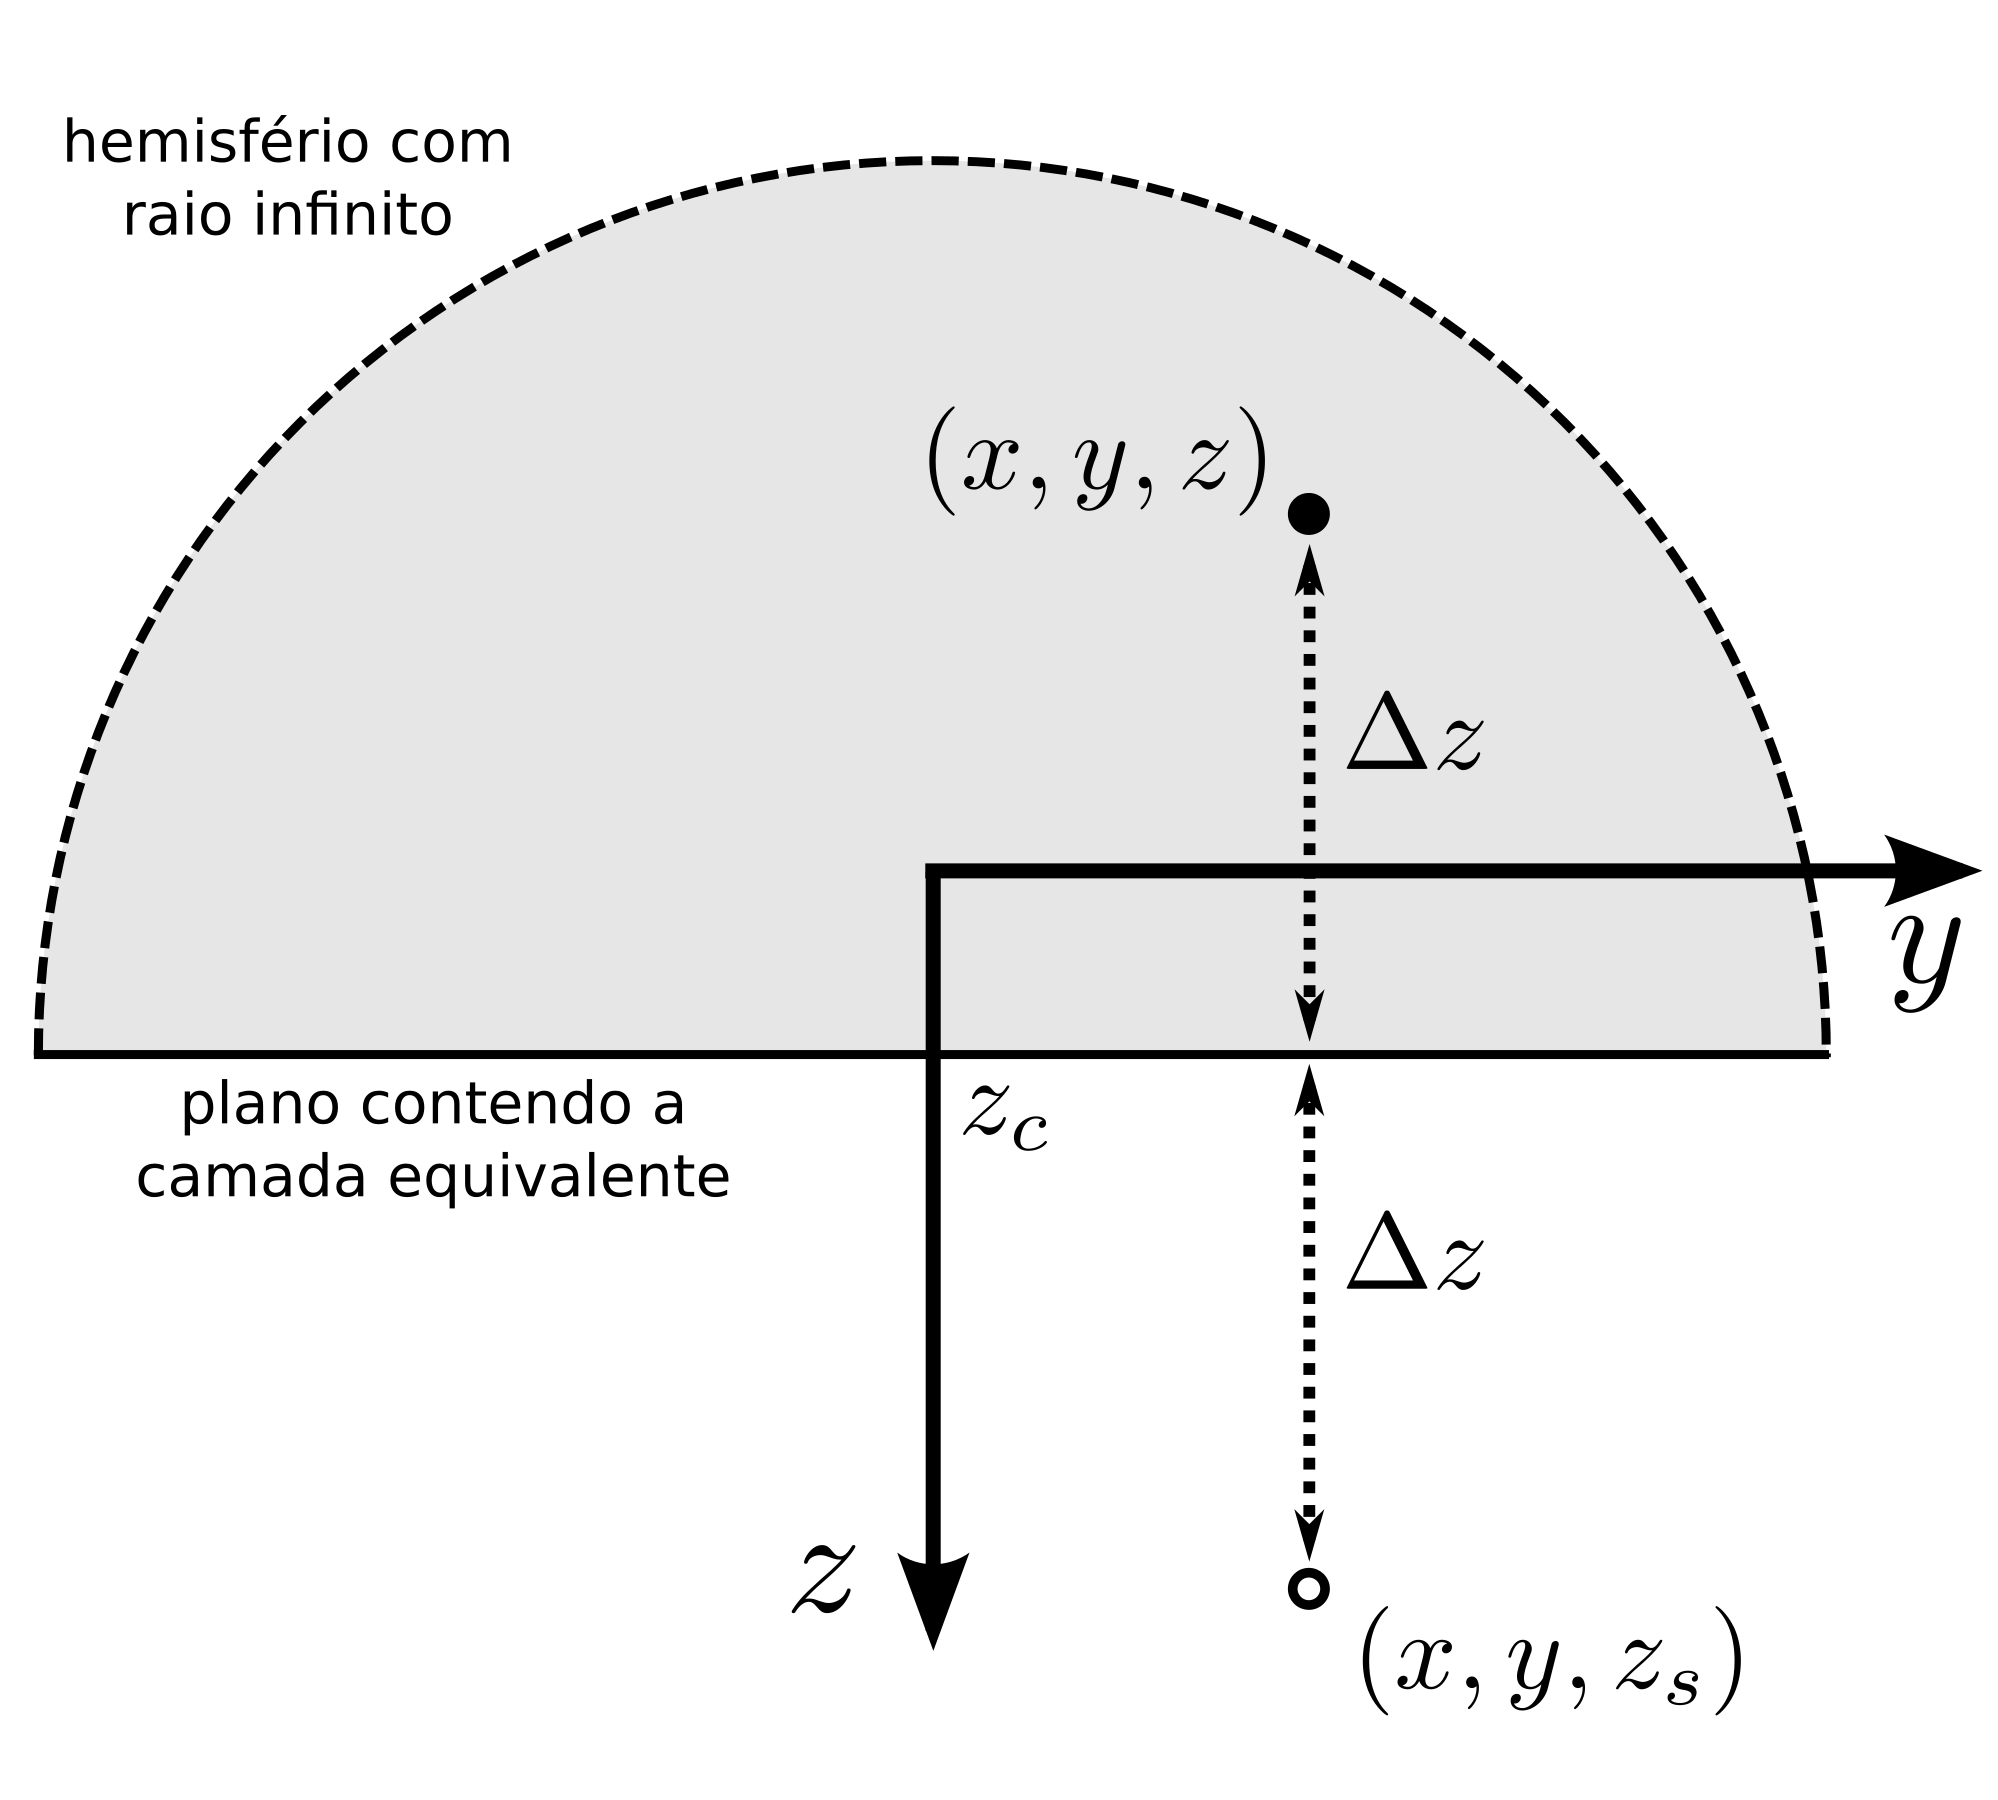
\includegraphics[width=0.75\textwidth]{Fig/eqlayer/surface_Green.png}
	\caption{ Representação 2D da superfícia utilizada para aplicar as identidades de Green. A superfície é formada por uma semi-esfera (linha traçejada) com raio infinito e o plano $z = z_{c}$ contendo a camada equivalente. Os pontos $(x, y, z)$ (ponto fechado) e $(x, y, z_{s})$ (ponto aberto) são posicionados simetricamente com respeito ao plano $z = z_{c}$ e definidos como $z = z_{c} - \Delta z$ e $z = z_{c} + \Delta z$, respectivamente.}
	\label{fig:surface_Green}
\end{figure}

O aspecto mais interessante sobre a distribuição de intensidades de momento magnético 
$p(x'', y'', z_{c})$ (equação \ref{eq:positivity_prop}) é que ela é definida como o produto de 
uma constante positiva $\frac{1}{2\pi}$ e a função $\partial_{z} \Omega(x'',y'',z_{c})$, que é 
estritamente positiva em todos os pontos $(x'',y'',z_{c})$ sobre a camada equivalente. 
Consequentemente, a função $p(x'', y'', z_{c})$ também é positiva em todos os pontos sobre a camada. 
Esta relação é similar àquela apresentada por \cite{pedersen1991} e \cite{li_etal_2014}. 
Aqueles autores determinaram, por meio de uma abordagem desenvolvida no domínio de Fourier, 
uma distribuição de intensidades de momento magnético positiva sobre uma camada equivalente 
contínua e com magnetização induzida na direção vertical. Eles também 
consideraram que a camada equivalente é plana, localizada em profundidade e é paralela 
ao plano horizontal que contem os dados observados de anomalia de campo total. 
Note que o presente trabalho não segue a abordagem no domínio de Fourier desenvolvida por aqueles 
autores. Além disso, a equação \ref{eq:positivity_prop} generaliza a condição de positividade dos 
momentos magnéticos por que (1) é válida para todos os casos nos quais a magnetização da camada 
equivalente tem a mesma direção da magnetização total das fontes, sendo ela puramente induzida ou não, 
e (2) não requer que os dados observados de anomalia de campo total estejam sobre um plano.


%%% Discretizing layer
\section{Parametrização e o problema direto}
\label{sec:par_prob_dir}

\subsection{Para a anomalia de campo total}
\label{subsec:tf_prob_dir}

Em situações práticas, não é possível determinar uma distribuição contínua de momentos magnéticos 
$p(x'',y'',z_{c})$ (equação \ref{eq:positivity_prop}) sobre a camada equivalente. Por esta razão, a 
camada é aproximada por um conjunto discreto de $M$ dipolos (fontes equivalentes) localizados no plano 
$z = z_{c}$ (Figura \ref{fig:eqlayer_tfa_sketch}). A anomalia de campo total produzida por esta camada 
discreta (anomalia de campo total predita) no ponto $(x_{i},y_{i},z_{i})$, $i=1,\dots,N$, é dada por 
\begin{equation}
\Delta T_{i}(\mathbf{s}) = \mathbf{g}_{i}(\mathbf{q})^{\top} \mathbf{p},
\label{eq:tfa_pred_i}
\end{equation}
em que $\mathbf{s}$ é um vetor $(M + 2) \times 1$ particionado dado por 
\begin{equation}
      \mathbf{s} = \begin{bmatrix}
		\mathbf{p} \\
		\mathbf{q}
	\end{bmatrix} \: ,
	\label{eq:s-vector}
\end{equation}
$\mathbf{q}$ é um vetor $2 \times 1$ definido em termos da inclinação e declinação ($I$ e $D$) 
da magnetização total na camada equivalente (vetor de direção de magnetização)
\begin{equation}
\mathbf{q} = \begin{bmatrix}
I \\ D 
\end{bmatrix} \: ,
\label{eq:q-vector}
\end{equation}
$\mathbf{p}$ é um vetor $M \times 1$ (vetor de momentos magnéticos) cujo $j$-ésimo elemento, $j=1,\dots,M$, 
é a intensidade do momento magnético $p_{j}$ (em $A \, m^{2}$) do $j$-ésimo dipolo e 
$\mathbf{g}_{i} (\mathbf{q})$ é outro vetor $M \times 1$ cujo $j$-ésimo elemento é definido pela função harmônica 
\begin{equation}
g_{ij} (\mathbf{q})  = \gamma_{m} \hat{\mathbf{u}}_{0}^T \, 
\mathbf{M}_{ij} \, \hat{\mathbf{u}}(\mathbf{q}) \: .
\label{eq:g_ij}
\end{equation}
Nesta equação, $\hat{\mathbf{u}}_{0} \equiv \hat{\mathbf{u}}(I_{0}, D_{0})$ e 
$\hat{\mathbf{u}}(\mathbf{q}) \equiv \hat{\mathbf{u}}(I, D)$ são vetores unitários
definidos pela equação \ref{eq:u-hat} em função da inclinação e declinação do 
campo principal ($I_{0}$ e $D_{0}$) e da camada equivalente ($I$ e $D$),
respectivamente, e $\mathbf{M}_{ij}$ é uma matriz $3 \times 3$ dada por 
\begin{equation}
\mathbf{M}_{ij} = \begin{bmatrix}
\partial_{xx} \frac{1}{r''} & 
\partial_{xy} \frac{1}{r''} &
\partial_{xz} \frac{1}{r''} \\
\partial_{xy} \frac{1}{r''} & 
\partial_{yy} \frac{1}{r''} &
\partial_{yz} \frac{1}{r''} \\
\partial_{xz} \frac{1}{r''} & 
\partial_{yz} \frac{1}{r''} &
\partial_{zz} \frac{1}{r''}
\end{bmatrix} \quad ,
\label{eq:Mij-matrix}
\end{equation}
em que $\partial_{\alpha\beta} \frac{1}{r''} \equiv \frac{\partial^{2}}{\partial \alpha \partial \beta} \frac{1}{r''}$ 
representa a segunda derivada da função $\frac{1}{r''}$ (equação \ref{eq:inv-r''}) em relação a $\alpha$ e $\beta$, 
$\alpha = x, y, z$ e $\beta = x, y, z$, avaliada nas coordenadas $(x, y, z) = (x_{i}, y_{i}, z_{i})$ do $i$-ésimo dado  
observado e $(x'', y'', z_{c}) = (x_{j}, y_{j}, z_{c})$ da $j$-ésima fonte equivalente.
As equações $\ref{eq:tfa_pred_i}$-$\ref{eq:Mij-matrix}$ mostram que a anomalia de campo total predita 
$\Delta T_{i}(\mathbf{s})$ possui uma relação linear com o vetor de momentos magnéticos $\mathbf{p}$ e uma 
relação não linear com o vetor de direção de magnetização $\mathbf{q}$ (equação \ref{eq:q-vector}).

%% Figura 

\begin{figure}[H]
	\centering
	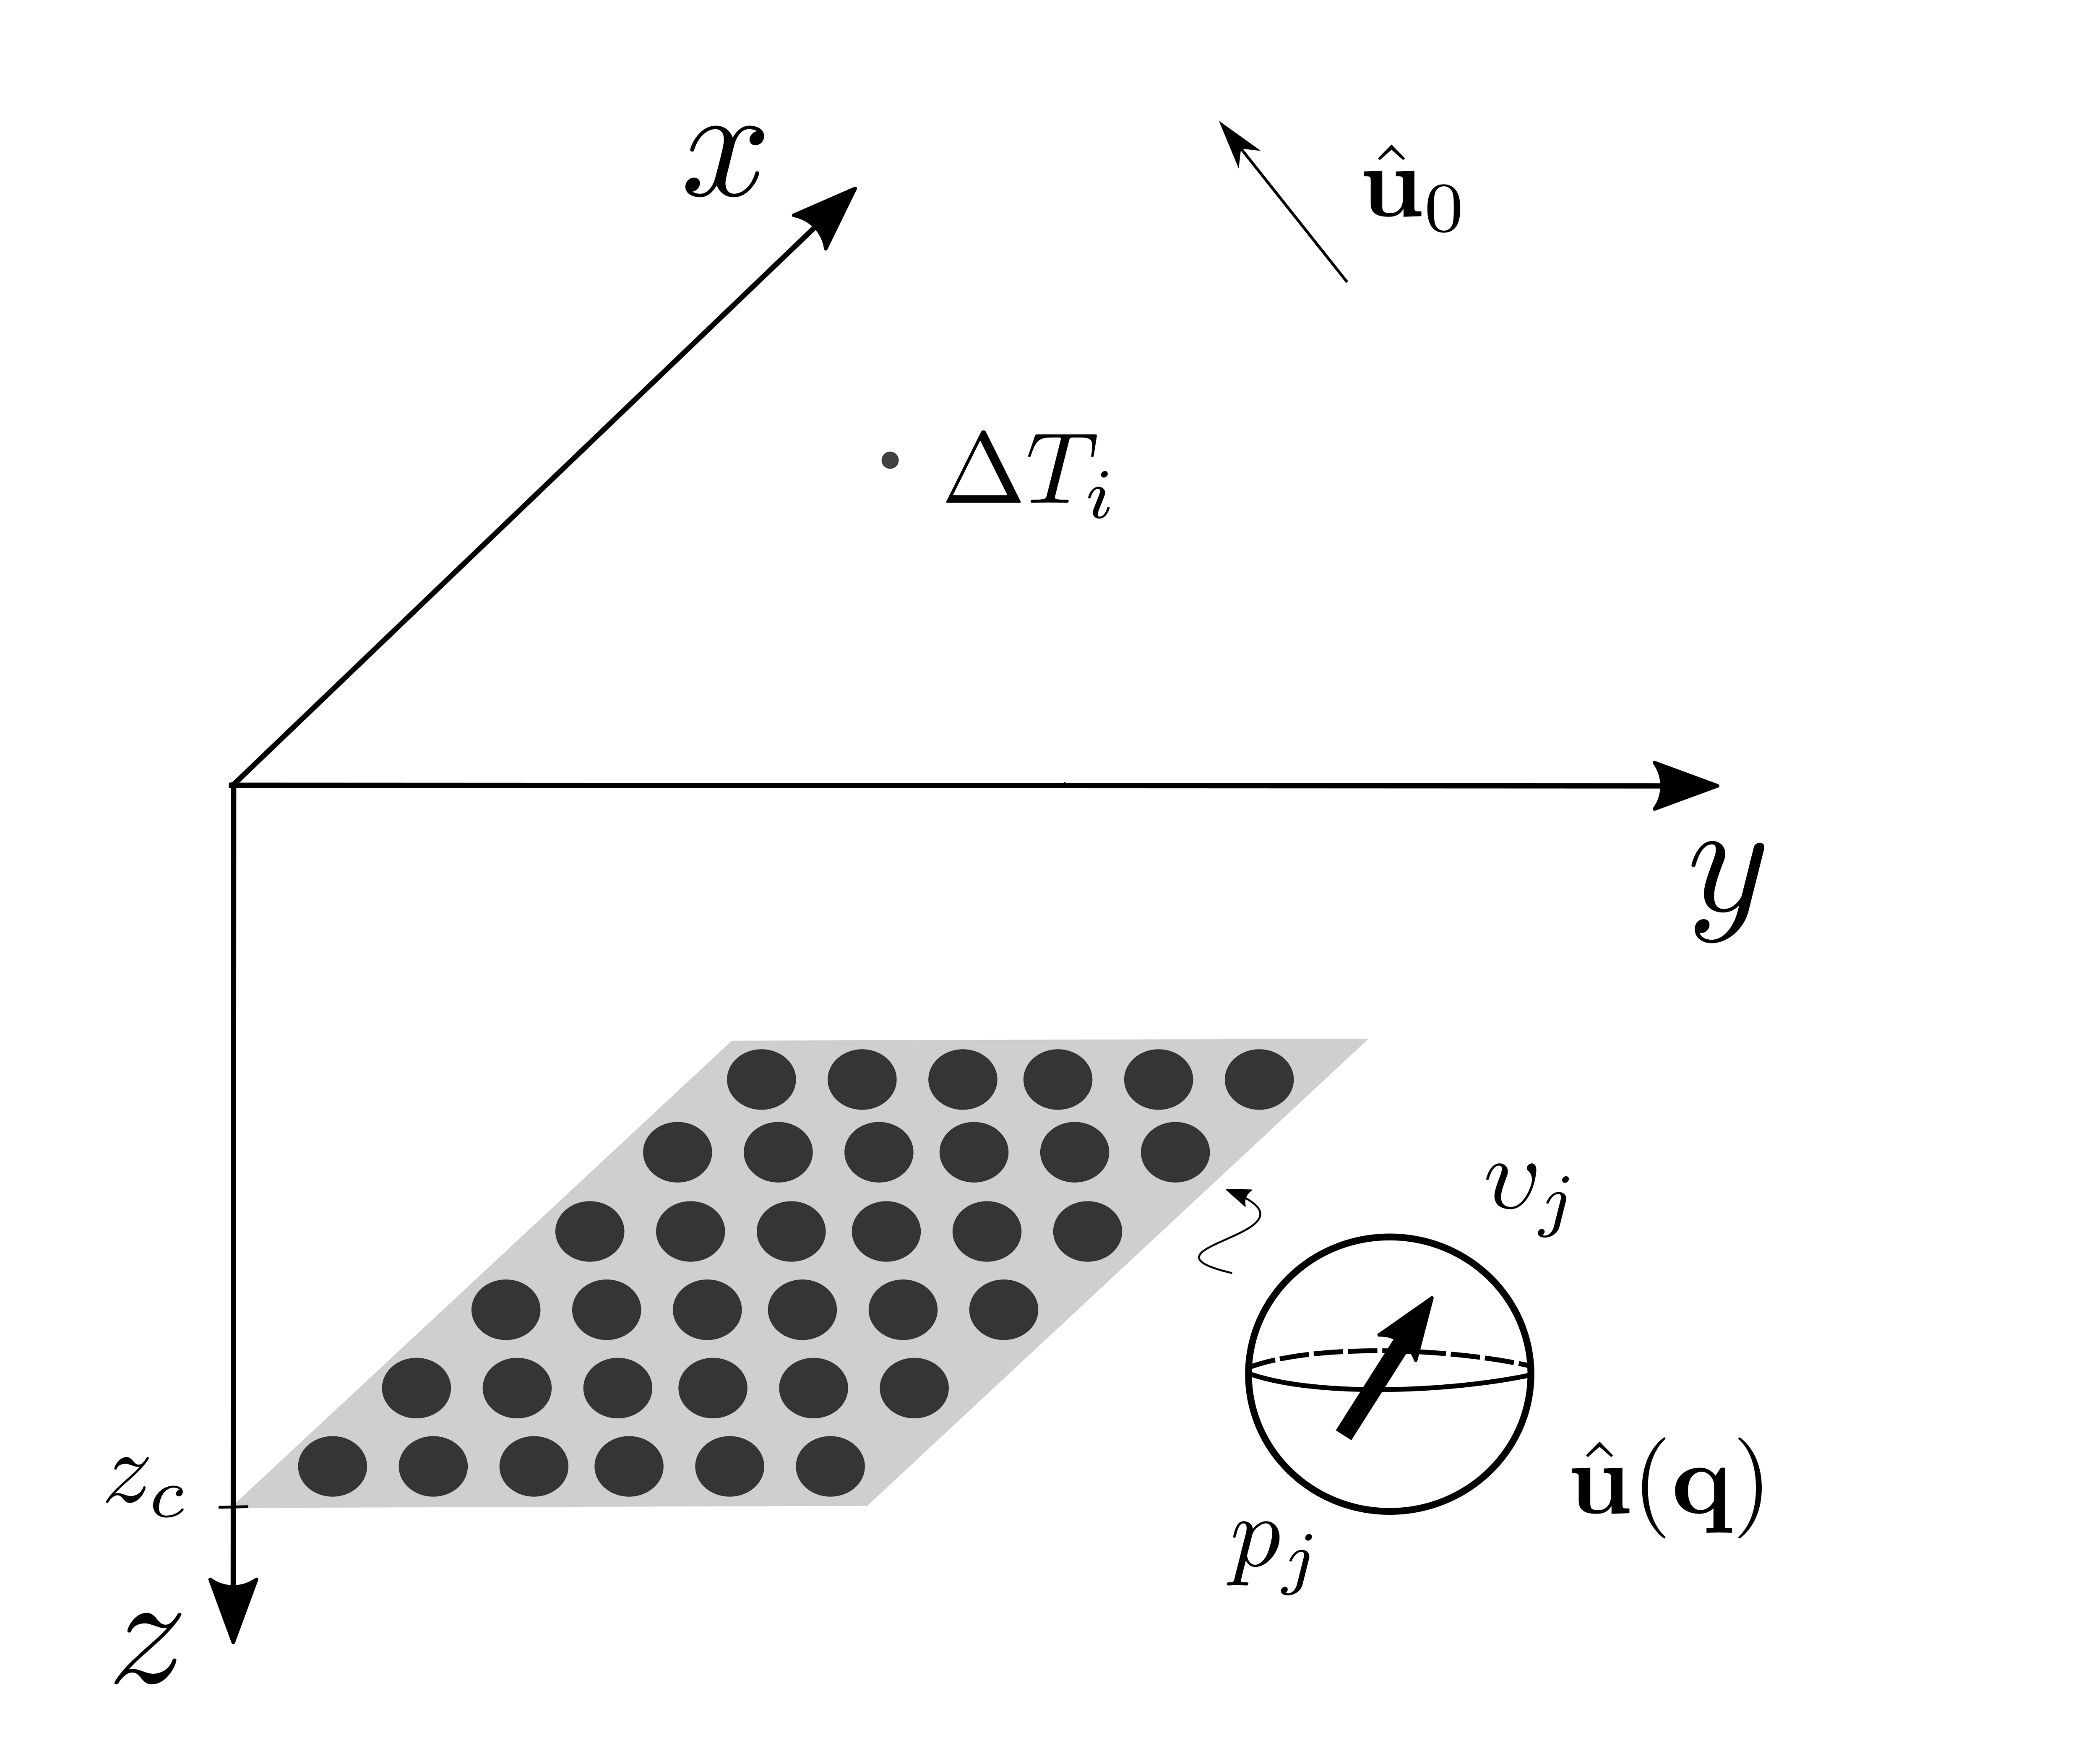
\includegraphics[width=.7\textwidth]{Fig/eqlayer/eqlayer_figure_tfa.png}
	\caption{Representação esquemática da camada equivalente para a anomalia de campo total. A camada é posicionada 
	sobre o plano horizontal a uma profundidade $z=z_{c}$. $\Delta T_{i}$ é a anomalia de campo total predita no ponto 
	$(x_{i},y_{i},z_{i})$ produzida pelo conjunto de $M$ fontes equivalentes (pontos pretos). Cada fonte é localizada 
	no ponto  $(x_{j},y_{j},z_{c})$, $j = 1, \dots, M$, e são representadas por um dipolo de volume unitário 
	$\upsilon_{j}$ com direção de magnetização $\hat{\mathbf{u}}(\mathbf{q})$ e momento magnético $p_{j}$. 
	$\hat{\mathbf{u}}_{0}$ é um vetor unitário na direção do campo principal.}
	\label{fig:eqlayer_tfa_sketch}
\end{figure}

\subsection{Para a componente vertical do campo magnético}
\label{subsec:bz_prob_dir}

De forma análoga a seção \ref{subsec:tf_prob_dir}, a componente vertical do campo de indução magnética (componente vertical predita) produzida por uma camada discreta posicionada a uma profundidade constante $z=z_c$ no ponto $(x_i,y_i,z_i)$, $i=1,\dots,N$, (Figura \ref{fig:eqlayer_bz_sketch}) é dada por 

\begin{equation}
B_{zi} (\mathbf{s})  = \mathbf{g}_{i}^{z}(\mathbf{q})^{\top} \, \mathbf{p},
\label{eq:pred_data_ith-z}
\end{equation}
em que $\mathbf{s}$ é um vetor $(M + 2) \times 1$ particionado (vetor de dados preditos) dado por 

\begin{equation}
      \mathbf{s} = \begin{bmatrix}
		\mathbf{p} \\
		\mathbf{q}
	\end{bmatrix} \: ,
	\label{eq:parameter-vector-z}
\end{equation}
$\mathbf{q}$ é o vetor direção de magnetização (equação \ref{eq:q_vetor}), $\mathbf{p}$ é um vetor $M \times 1$ (vetor de momentos magnéticos) cujo $j$-ésimo elemento, $j=1,\dots,M$, é a intensidade do momento magnético $p_{j}$ (em $A \, m^{2}$) dos $j$-ésimo dipolo e $\mathbf{g}_{i}^{z} (\mathbf{q})$ é outro vetor $M \times 1$ cujo $j$-ésimo elemento é definido pela função harmônica 

\begin{equation}
g_{ij}^{z}(\mathbf{q})  = \gamma_m \, \mathbf{M}_{ij}^{z^\top} \, \hat{\mathbf{m}}(\mathbf{q}) \: .
\label{eq:g_ij-z}
\end{equation}
Nesta equação, $\mathbf{M}_{ij}^{z^\top}$ é um vetor $1 \times 3$ dada por 

\begin{equation}
\mathbf{M}_{ij}^{z^\top} = \begin{bmatrix}
\partial_{xz} \frac{1}{r} & 
\partial_{yz} \frac{1}{r} &
\partial_{zz} \frac{1}{r}
\end{bmatrix}^\top \quad ,
\label{eq:Mij-matrix-z}
\end{equation}
em que $\partial_{\alpha z} \frac{1}{r} \equiv \frac{\partial^{2}}{\partial \alpha \partial z} \frac{1}{r}$, representa a derivada segunda com respeito a $\alpha = x, y, z$, do inverso da distância $\frac{1}{r}$ (equação \ref{eq:inverse-distance}) entre as coordenadas de observação $(x, y, z) = (x_{i}, y_{i}, z_{i})$ e as coordenadas das fontes equivalentes $(x'', y'', z_{c}) = (x_{j}, y_{j}, z_{c})$. Note que, analogamente a seção \ref{subsec:tf_prob_dir}, a componente vertical do campo $B_{zi}(\mathbf{s})$ possui uma relação linear com o vetor de momentos magnéticos $\mathbf{p}$ e uma relação não linear com o vetor de direção de magnetização $\mathbf{q}$ (equação \ref{eq:q_vetor}).

%% Figura
\begin{figure}[H]
	\centering
	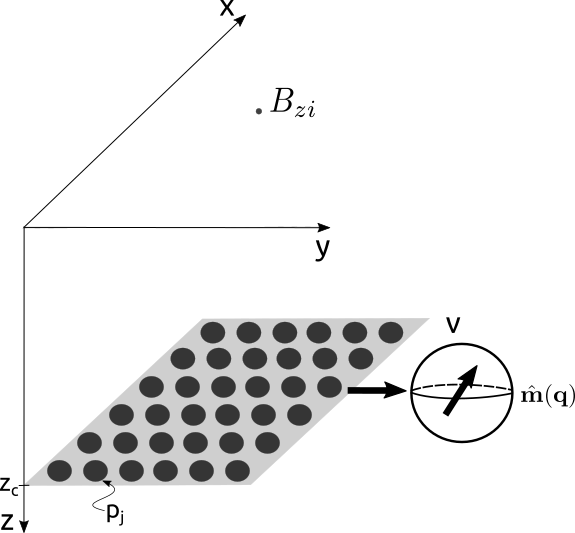
\includegraphics[width=.7\textwidth]{Fig/mag_vec/eqlayer_figure_bz.png}
	\caption{Representação esquemática da camada equivalente para a componente vertical do campo magnético. A camada também é posicionada sobre o plano horizontal a uma profundidade $z=z_c$, de forma similar para a anomalia de campo total (Figura \ref{fig:eqlayer_tfa_sketch}). $B_{zi}$ é a componente vertical do campo magnético predita no ponto $(x_i,y_i,z_i)$ produzida pelo conjunto de $M$ fontes equivalentes (pontos pretos). Cada fonte é localizada no ponto  $(x_j,y_j,z_c)$, $j = 1,\hdots, M$, e são representadas por um dipolo de volume unitário $\upsilon$ com direção de magnetização $\hat{\mathbf{m}}(\mathbf{q})$ e momento magnético $p_j$.}
	\label{fig:eqlayer_bz_sketch}
\end{figure}

PAREI AQUI

\section{Problema inverso}

\subsection{A estimativa da direção de magnetização}
\label{subsec:mag_dir_est}

%%%%% Defining the objective function
Seja $\mathbf{\Delta T}^{o}$ o vetor de dados observados cujo $i$-ésimo elemento $\Delta T_{i}^{o}$ é a anomalia de campo total produzida por uma fonte magnética no ponto $(x_{i},y_{i},z_{i})$, $i = 1, \dots, N$. Similarmente, seja $\mathbf{\Delta T} (\mathbf{s})$ o vetor de dados preditos cujo $i$-ésimo elemento $\Delta T_{i}(\mathbf{s})$ (equação \ref{eq:tfa_pred_i}) é a anomalia de campo total produzida por uma camada equivalente discreta no mesmo ponto $(x_{i},y_{i},z_{i})$. Com o objetivo de estimarmos um vetor de parâmetros $\mathbf{s}$ (equação \ref{eq:parameter-vector}) que minimiza a diferença entre $\mathbf{\Delta T}^{o}$ e $\mathbf{\Delta T}(\mathbf{s})$, temos que resolver o problema inverso:

\begin{subequations}
	\begin{align}
	& \text{minimizar}
	& &\Psi(\mathbf{s}) =\lVert \mathbf{\Delta T}^{o} - \mathbf{\Delta T} (\mathbf{s}) 
	\rVert_{2}^{2} + \, \mu f_0 \parallel \mathbf{p} \parallel_{2}^{2} \: , \\
	& \text{sujeito a}
	& & \mathbf{p} \geqslant \mathbf{0} \: .
	\end{align}
	\label{eq:positivity_goal_function}
\end{subequations}
O primeiro e o segundo termo da equação \ref{eq:positivity_goal_function}a são, respectivamente, a função de ajuste e a função regularizadora de Tikhonov de ordem zero, $\mu$ é o parâmetro de regularização, $\| \cdot \|_{2}^{2}$ representa o quadrado da norma Euclidiana e $f_{0}$ é um fator de normalização. Na inequação \ref{eq:positivity_goal_function}b, $\mathbf{0}$ é um vetor $M \times 1$ com todos os elementos iguais a zero no qual o sinal da inequação é aplicado elemento a elemento. Este vínculo de positividade sobre o vetor de momentos magnéticos $\mathbf{p}$ é incorporado utilizando o chamado \textit{estimador de mínimos quadrados não negativo} ou somente NNLS (do inglês \textit{Nonnegative least squares}) proposto por \cite{lawson_hanson_1974}.

Para resolver este problema inverso, temos que considerar primeiramente uma expansão até segunda ordem da função objetivo (equação \ref{eq:positivity_goal_function}a) em torno de $\mathbf{s} = \mathbf{s}^{k}$ (equação \ref{eq:parameter-vector}):

\begin{equation}
\Psi(\mathbf{s}^{k} + \mathbf{\Delta s}^{k}) \approx \Psi(\mathbf{s}^{k}) + 
{\mathbf{J}^{k}}^{\top} \mathbf{\Delta s}^{k} + 
\frac{1}{2} {\mathbf{\Delta s}^{k}}^{\top} \mathbf{H}^{k} \mathbf{\Delta s}^{k}  \: ,
\label{eq:sec_ord_goal}
\end{equation}
em que $\mathbf{\Delta s}^{k}$ é uma perturbação no vetor de parâmetros e os termos $\mathbf{J}^{k}$ e $\mathbf{H}^{k}$ são, respectivamente, o vetor gradiente e a matriz Hessiana avaliadas em $\mathbf{s}^{k}$. Então, estimamos o vetor de perturbação $\bar{\mathbf{\Delta s}}^k$ que minimiza a função expandida (equação \ref{eq:sec_ord_goal}) tomando o seu gradiente e igualando o resultado ao vetor nulo. Este procedimento nos leva ao sistema linear 

\begin{equation}
\mathbf{H}^{k} \bar{\mathbf{\Delta s}}^{k} = - \mathbf{J}^{k} \: ,
\label{eq:linear_sys_GN}
\end{equation}
que representa o $k$-ésimo passo do método de Gauss-Newton \citep{aster2005} para a minimização da função objetivo (equação \ref{eq:positivity_goal_function}a). Reescrevemos este sistema linear desprezando as derivadas cruzadas na matriz Hessiana como: 

\begin{equation}
\left[
\begin{array}{c|c}
\mathbf{H}_{pp}^{k} & \mathbf{0} \\
\hline
\mathbf{0}^{\top} & \mathbf{H}_{qq}^{k}
\end{array}
\right] \left[ \begin{array}{c}
\bar{\mathbf{\Delta p}}^{k} \\ 
\bar{\mathbf{\Delta q}}^{k} 
\end{array} \right] \approx -\left[ \begin{array}{c}
\mathbf{J}_{p}^{k} \\ 
\mathbf{J}_{q}^{k} 
\end{array} \right] ,
\label{eq:linear_sys_GN_block}
\end{equation}
em que $\mathbf{0}$ é uma matriz $M \times 2$ que contém todos os elementos iguais a zero, $\bar{\mathbf{\Delta p}}^{k} = \bar{\mathbf{p}}^{k+1} - \bar{\mathbf{p}}^{k}$ é a correção no vetor de momentos magnéticos $\mathbf{p}$, $\bar{\mathbf{\Delta q}}^{k} = \bar{\mathbf{q}}^{k+1} - \bar{\mathbf{q}}^{k}$ é a correção no vetor direção de magnetização e os termos $\mathbf{J}_{\alpha}^{k}$ e $\mathbf{H}_{\alpha \alpha}^{k}$, $\alpha = p,q$, são os vetores gradientes e as matrizes Hessianas calculadas com respeito aos elementos dos $\mathbf{p}$ e $\mathbf{q}$, respectivamente. 

O vetor gradiente $\mathbf{J}_{p}^{k}$ e a matriz Hessiana $\mathbf{H}_{pp}^{k}$ (equação \ref{eq:linear_sys_GN_block}) relativas ao vetor de momentos magnéticos $\mathbf{p}$ (equação \ref{eq:parameter-vector}) são, respectivamente, 

\begin{equation}
\mathbf{J}_{p}^{k} = -2 {\mathbf{G}_{p}^{k}}^{\top} 
\left[ \mathbf{\Delta T}^{o} - \mathbf{\Delta T} (\bar{\mathbf{s}}^{k}) \right] + 
2\mu f_{0}^{k} \bar{\mathbf{p}}^{k} 
\label{eq:grad_p}
\end{equation}
e 

\begin{equation}
\mathbf{H}_{pp}^{k} = 2 {\mathbf{G}_{p}^{k}}^{\top} \mathbf{G}_{p}^{k} + 
2 \mu f_{0}^{k} \mathbf{I} \: ,
\label{eq:hess_p}
\end{equation}
em que $\mathbf{G}_p^{k}$ é uma matriz de dimensão $N \times M$ cujo $ij$-ésimo elemento é dado pela função harmônica $g_{ij}(\bar{\mathbf{q}}^{k})$ (equação \ref{eq:g_ij}) avaliada na direção de magnetização $\bar{\mathbf{q}}^{k}$, $\mathbf{I}$ é uma matriz identidade de dimensão $M \times M$ e $f_{0}^{k}$ é um fator de normalização igual a 

\begin{equation}
f_{0}^{k} = \dfrac{trace \left({\mathbf{G}_{p}^{k}}^{\top} \mathbf{G}_{p}^{k} \right)}{M} \, .
\label{eq:norm_factor}
\end{equation}

O vetor gradiente $\mathbf{J}_{q}^{k}$ e a matriz Hessiana $\mathbf{H}_{qq}^{k}$ (equação \ref{eq:linear_sys_GN_block}) relativas a direção de magnetização $\mathbf{q}$ (equação \ref{eq:q_vetor}) são, respectivamente, 

\begin{equation}
\mathbf{J}_{q}^{k} = -2 {\mathbf{G}_{q}^{k}}^{\top} 
\left[ \mathbf{\Delta T}^{o} - \mathbf{\Delta T} (\bar{\mathbf{s}}^{k}) \right]
\label{eq:grad_q}
\end{equation}
e

\begin{equation}
\mathbf{H}_{qq}^{k} \approx 2 {\mathbf{G}_{q}^{k}}{^\top} \mathbf{G}_{q}^{k} \: ,
\label{eq:hess_q}
\end{equation}
em que $\mathbf{G}_{q}^{k}$ é uma matriz $N \times 2$ dada por 

\begin{equation}
\mathbf{G}_{q}^{k} = \begin{bmatrix}
\partial_{I} \mathbf{g}_{1}(\bar{\mathbf{q}}^{k})^{\top} \bar{\mathbf{p}}^{k} & 
\partial_{D} \mathbf{g}_{1}(\bar{\mathbf{q}}^{k})^{\top} \bar{\mathbf{p}}^{k} \\
\vdots & \vdots  \\
\partial_{I} \mathbf{g}_{N}(\bar{\mathbf{q}}^{k})^{\top} \bar{\mathbf{p}}^{k} & 
\partial_{D} \mathbf{g}_{N}(\bar{\mathbf{q}}^{k})^{\top} \bar{\mathbf{p}}^{k} 
\end{bmatrix} \: ,
\label{eq:Gq}
\end{equation}
em que $\partial_{\alpha} \mathbf{g}_{i}(\bar{\mathbf{q}}^{k}) \equiv \frac{\partial \mathbf{g}_{i}(\bar{\mathbf{q}}^{k})}{\partial \alpha}$, $\alpha= I, D$, representa a primeira derivada do vetor $\mathbf{g}_{i}(\bar{\mathbf{q}}^{k})$ (equação \ref{eq:tfa_pred_i}) com respeito a inclinação $I$ e a declinação $D$ da magnetização total das fontes.

\subsubsection{Processo iterativo para a estimativa da direção de magnetização}

A iteração $k=0$ do nosso algoritmo começa com uma aproximação inicial $\bar{\mathbf{q}}^{k} = \bar{\mathbf{q}}^{0}$ para o vetor direção de magnetização $\mathbf{q}$ (equação \ref{eq:q_vetor}). Utilizando esta aproximação inicial $\bar{\mathbf{q}}^{k}$, a parte superior da equação \ref{eq:linear_sys_GN_block} nos leva ao seguinte sistema linear para o vetor de momentos magnéticos:

\begin{equation}
\left[ {\mathbf{G}_{p}^{k}}^{\top} \mathbf{G}_{p}^{k} + 
\mu f_{0}^{k} \mathbf{I} \right] \bar{\mathbf{p}}^{k} = {\mathbf{G}_{p}^{k}}^{\top} \mathbf{\Delta T}^{o} \: .
\label{eq:linear_sys_p}
\end{equation}
Para impor o vínculo de positividade (equação \ref{eq:positivity_goal_function}b) sobre a distribuição de momentos magnéticos, este sistema linear é resolvido usando o método de NNLS \citep{lawson_hanson_1974, silvadias_etal_2010}. Esta distribuição de momentos magnéticos é então usada para estimar uma correção $\bar{\mathbf{\Delta q}}^{k}$ no vetor direção de magnetização resolvendo um sistema não linear utilizando o método de Levenberg-Marquardt \citep{aster2005}:

\begin{equation}
\left[ {\mathbf{G}_{q}^{k}}^{\top} \mathbf{G}_{q}^{k} + \lambda \, \mathbf{I} \right] 
\bar{\mathbf{\Delta q}}^{k} = {\mathbf{G}_{q}^{k}}^{\top} 
\left[ \mathbf{\Delta T}^{o} - \mathbf{\Delta T} (\mathbf{s}^{k}) \right] \: ,
\label{eq:linear_sys_q}
\end{equation}
em que $\lambda$ é o parâmetro de Marquardt e $\mathbf{I}$ é uma matriz identidade. Após estimarmos a correção $\bar{\mathbf{\Delta q}}^{k}$ na $k$-ésima iteração, atualizamos a direção de magnetização aplicando a correção a seguir:

\begin{equation}
\bar{\mathbf{q}}^{k+1} = \bar{\mathbf{q}}^{k} + \bar{\mathbf{\Delta q}}^{k} \: ,
\label{eq:q_next}
\end{equation}
e utilizando esta nova direção para estimar uma nova distribuição de momentos magnéticos com a equação \ref{eq:linear_sys_p} e assim sucessivamente. O processo iterativo é interrompido quando a função objetivo (equação \ref{eq:positivity_goal_function}a) é invariante ao longo de sucessivas iterações. Mostramos também que este método falha em situações nas quais as fontes são magnetizadas verticalmente (Apêndice \ref{append:vertical-magnetization}).

\subsection{O cálculo das componentes do campo magnético e a amplitude do campo}
\label{subsec:componentes_vec}

Seja $\mathbf{B}_{z}^{o}$ o vetor de dados observados cujo $i$-ésimo elemento $B_{zi}^{o}$ é a componente vertical do campo magnético produzida por uma fonte magnética no ponto $(x_{i},y_{i},z_{i})$, $i = 1, \dots, N$. Similarmente, seja $\mathbf{B}_{z}^{p} (\mathbf{s})$ o vetor de dados preditos cujo $i$-ésimo elemento $B_{zi}^{p}(\mathbf{s})$ (equação \ref{eq:pred_data_ith-z}) é a componente vertical do campo magnético produzida por uma camada equivalente discreta no mesmo ponto $(x_{i},y_{i},z_{i})$. Com o objetivo de minimizar a diferença entre $\mathbf{B}_{z}^{o}$ e $\mathbf{B}_{z}^{p} (\mathbf{s})$, temos que resolver a equação:

\begin{equation}
\Psi(\mathbf{s}) =\lVert \mathbf{B}_{z}^{o} - \mathbf{B}_{z}^{p} (\mathbf{s}) 
	\rVert_{2}^{2} + \, \mu  \parallel \mathbf{p} \parallel_{2}^{2} \: , \\
\label{eq:goal_function_vec}
\end{equation}
em que o primeiro e o segundo termo da equação \ref{eq:goal_function_vec} são a função de ajuste e a função regularizadora de Tikhonov de ordem zero, $\mu$ é o parâmetro de regularização e $\| \cdot \|_{2}^{2}$ representa o quadrado da norma Euclidiana. 

Assumimos neste caso que a camada equivalente depende somente do vetor de momentos magnéticos $\mathbf{p}$ e, portanto, devemos impor uma direção de magnetização $\mathbf{q}$ arbitrária sobre ela. Com isso, o sistema linear que iremos resolver é dado por:

\begin{equation}
\left[ \mathbf{G}_{z}^{\top} \mathbf{G}_{z} + \mu \mathbf{I} \right] \bar{\mathbf{p}} = \mathbf{G}_{z}^{\top} \mathbf{B}_{z}^{o} \: ,
\label{eq:linear_sys_p_z}
\end{equation}
em que $\mathbf{G}_{z}$ é uma matriz de dimensão $N \times M$ cujo $ij$-ésimo elemento é dado pela função harmônica $g_{ij}^{z}(\mathbf{q})$ (equação \ref{eq:g_ij-z}) avaliada na direção de magnetização fixa $\mathbf{q}$ e $\mathbf{I}$ é uma matriz identidade de dimensão $M \times M$. A equação \ref{eq:linear_sys_p_z} é denominada como estimador de mínimos quadrados \citep{aster2005}. Após estimarmos uma distribuição de momentos magnéticos $\bar{\mathbf{p}}$ relativa a uma direção de magnetização arbitrária $\mathbf{q}$, calculamos as outras duas componentes do campo magnético aplicando a relação dada por:

\begin{equation}
\mathbf{B}_{x}^{p}  = \mathbf{G}_{x} \bar{\mathbf{p}}
\label{eq:pred_vec_x}
\end{equation}
e

\begin{equation}
\mathbf{B}_{y}^{p}  = \mathbf{G}_{y} \bar{\mathbf{p}}
\label{eq:pred_vec_y}
\end{equation}
em que $\mathbf{B}_{x}^{p}$ e $\mathbf{B}_{y}^{p}$ são, respectivamente, os vetores de dados preditos com dimensão $N \times 1$ das componentes $x$ e $y$ do campo de indução magnética. As matrizes $\mathbf{G}_{x}$ e $\mathbf{G}_{y}$ possuem dimensão $N \times M $ cujo os elementos são dados por: 

\begin{equation}
g_{ij}^{x}(\mathbf{q})  = \gamma_m \, \mathbf{M}_{ij}^{x^\top} \, \hat{\mathbf{m}}(\mathbf{q}) \: 
\label{eq:g_ij-x}
\end{equation}
e 
\begin{equation}
g_{ij}^{y}(\mathbf{q})  = \gamma_m \, \mathbf{M}_{ij}^{y^\top} \, \hat{\mathbf{m}}(\mathbf{q}) \: ,
\label{eq:g_ij-y}
\end{equation}
em que 

\begin{equation}
\mathbf{M}_{ij}^{x^\top} = \begin{bmatrix}
\partial_{xx} \frac{1}{r} & 
\partial_{xy} \frac{1}{r} &
\partial_{xz} \frac{1}{r}
\end{bmatrix}^\top \quad 
\label{eq:Mij-matrix-x}
\end{equation}
e 

\begin{equation}
\mathbf{M}_{ij}^{y^\top} = \begin{bmatrix}
\partial_{xy} \frac{1}{r} & 
\partial_{yy} \frac{1}{r} &
\partial_{yz} \frac{1}{r}
\end{bmatrix}^\top \quad .
\label{eq:Mij-matrix-y}
\end{equation}
As derivadas $\partial_{\alpha\beta} \frac{1}{r} \equiv \frac{\partial^{2}}{\partial \alpha \partial \beta} \frac{1}{r}$, representam as derivadas segundas com respeito a $\alpha = x, y$ e $\beta = x, y, z$, do inverso da distância $\frac{1}{r}$ (equação \ref{eq:inverse-distance}) entre as coordenadas de observação $(x, y, z) = (x_{i}, y_{i}, z_{i})$ e as coordenadas das fontes equivalentes $(x'', y'', z_{c}) = (x_{j}, y_{j}, z_{c})$. Além disso, calculamos a amplitude do campo magnético aplicando a relação

\begin{equation}
\mathbf{B}_a = \sqrt{ \mathbf{B}_{x}^{p^2} + \mathbf{B}_{y}^{p^2} + \mathbf{B}_{z}^{p^2}}   
\label{eq:amplitude_field}
\end{equation}
em que $\mathbf{B}_{x}^{p}$, $\mathbf{B}_{y}^{p}$ e $\mathbf{B}_{z}^{p}$ são as componentes do campo magnético e $\mathbf{B}_a$ é a vetor amplitude do campo magnético. 

\section{A escolha da profundidade da camada ($\mathbf{z_{c}}$) e do parâmetro de regularização ($\mathbf{\mu}$)}

O procedimento pelo qual utilizamos a camada equivalente para estimar a direção de magnetização total das fontes magnéticas e o cálculo das componentes do campo magnético requer a escolha de dois parâmetros principais. O primeiro é a profundidade da camada $z_c$ (Figuras \ref{fig:eqlayer_tfa_sketch} e \ref{fig:eqlayer_bz_sketch}) e o segundo é o parâmetro de regularização $\mu$ mostrado na equação \ref{eq:linear_sys_p}. 

O método utilizado para a escolha da profundidade da camada é baseado na abordagem clássica proposta por \cite{dampney1969}. O autor aponta que o posicionamento da camada deve satisfazer um intervalo de $2,5$ a $6,0$ vezes o espaçamento dos dados. Vale ressaltar que esta regra foi aplicada pelos autores em uma grade com dados regularmente espaçados. Contudo, a escolha para aplicar nosso método corresponde a um intervalo de $2$ a $3$ vezes o valor do maior espaçamento entre os dados. É necessário lembrar que este intervalo foi encontrado empiricamente. 

Para resolver a equação \ref{eq:linear_sys_p}, temos que escolher um valor confiável para o parâmetro de regularização. Com este propósito, usamos o método da curva-L, que serve como uma filtragem de ruídos dos dados, sem que o resultado final perca informações. O 'cotovelo' desta curva é o valor ótimo de parâmetro no qual é feito o balanço entre a função de ajuste e a função regularizadora. 